\section{Considerações iniciais}

\textit{Deep learning}, ou aprendizado profundo em português, é um ramo do aprendizado de máquina que por sua vez é uma das áreas de estudo nas ciências de inteligência artificial. 
Segundo \citeonline{Simon2013od}, o aprendizado de máquina tem um foco maior em algoritmos de computação que possuem a capacidade de aprenderem e se aprimorarem, sem a necessidade de uma programação expressa.
A partir disso, o \textit{deep learning} tenta alcançar esse ato de educar-se a partir de repetidas iterações dentro de um ambiente correspondente à um objetivo em particular, dessa forma encontrando um resultado para tal objetivo através de reflexões de seus erros em novas tentativas.

\section{Aprendizado de máquina}

O aprendizado de máquina é uma área de estudo da inteligência artificial que se dedica a desenvolver aplicações capazes de produzir resultados a partir de entradas de dados. 
Através de processamentos realizados por máquinas, busca-se aprimorar o resultado até se atingir um patamar ótimo de desempenho. 
É fundamental que essa aprendizagem seja realizada exclusivamente pela máquina, com no máximo o auxílio ou supervisão humana, conforme destacado por \citeonline{ed2021}.

Alguns exemplos da utilização de aprendizado de máquina em nosso cotidiano são motores de busca da Internet como Google e Netflix, que a partir de buscas anteriores, consegue descobrir o que o  usuário tem mais interesse e a partir disso encontrar resultados que satisfaçam o usuário.
Para mais, já existem aplicações do aprendizado de máquina no campo comercial, industrial e até mesmo agrícola, que utilizada junto com visão computacional para detecção de doenças e pragas, controle de safra e na avaliação não invasiva de atributos como qualidade, aparência e volume \cite{agrivis2020}.

Para alcançar o aprendizado, existem certas abordagens que o programador pode seguir para implementar o algoritmo requerido e obter uma boa acurácia. 
Atualmente pode-se dividir tais abordagens em quatro diferentes métodos: Supervisionado, não supervisionado, semi-supervisionado e por reforço \cite{Russell2009}.

O aprendizado supervisionado se refere aos casos onde há um provedor que ativamente provê o algoritmo de aprendizagem de máquina com dados de treino já rotulados e definem quais serão as variáveis esperadas de resultado. 
Logo, o algoritmo possui desde o início sua entrada e saída pré-estabelecida e precisa aprender como realizar a transformação da entrada à saída \cite{Russell2009}.
Exemplos desse método são algoritmos de regressão e classificação.

De acordo com \citeonline{geeron2017handson}, o aprendizado não supervisionado é uma abordagem de aprendizado de máquina em que o algoritmo é alimentado com dados não rotulados e é deixado para identificar padrões ou estruturas por conta própria. 
Ao contrário do aprendizado supervisionado, em que o algoritmo recebe dados rotulados e é treinado para fazer previsões com base nesses rótulos, no aprendizado não supervisionado não há informações prévias sobre as classes ou categorias dos dados. 
Em vez disso, o algoritmo é responsável por encontrar grupos ou segmentos nos dados que possuem características semelhantes. 
Essa abordagem é amplamente utilizada em tarefas de análise de dados, como \textit{clustering} e redução de dimensionalidade, e é especialmente útil quando não se tem informações suficientes ou claras sobre os dados.

Ainda de acordo com \citeonline{geeron2017handson}, o aprendizado semi-supervisionado é uma abordagem que se situa entre o aprendizado supervisionado e o não supervisionado. 
Nesse tipo de aprendizado, o modelo tem acesso tanto a um conjunto de dados rotulados quanto a um conjunto de dados não rotulados. 
A ideia é que, ao treinar o modelo com os dados rotulados, ele seja capaz de aprender a classificar novos dados com base nesses rótulos conhecidos. 
Por sua vez, ao treinar o modelo com os dados não rotulados, ele é exposto a padrões e estruturas que não seriam tão facilmente identificáveis com apenas os dados rotulados. 
Dessa forma, o aprendizado semi-supervisionado é uma abordagem que pode ajudar a melhorar a performance do modelo, principalmente quando o conjunto de dados rotulados é escasso ou quando o processo de rotulação é custoso ou complexo.

O aprendizado por reforço é uma técnica de aprendizado de máquina em que um agente aprende a tomar decisões a partir de suas interações com um ambiente. 
O objetivo é maximizar uma recompensa cumulativa que é recebida pelo agente por suas ações ao longo do tempo. 
O agente pode observar o estado atual do ambiente e tomar uma ação, que altera o estado do ambiente e gera uma recompensa. 
O aprendizado por reforço é frequentemente usado em problemas de tomada de decisão sequencial, como jogos, controle de robôs e sistemas de recomendação. 
Ele utiliza técnicas de otimização para determinar a política de ações do agente que maximiza a recompensa cumulativa ao longo do tempo \cite{geeron2017handson}.

Por melhor que seja o desempenho do aprendizado de máquina em diversas áreas, a sua maior desvantagem é a dependência de dados de treinamento de alta qualidade. 
Sem uma quantidade significativa de dados precisos, o modelo pode ser insuficiente ou produzir resultados imprecisos \cite{geeron2017handson}. 
Isso pode se tornar um obstáculo significativo para empresas e organizações que não têm acesso a grandes volumes de dados ou não possuem recursos para coletar, rotular e limpar dados. 
Além disso, os algoritmos de aprendizado de máquina podem ser enviesados, e reproduzir preconceitos presentes nos dados de treinamento, o que pode ter consequências graves em áreas como justiça criminal, saúde e finanças. 
Por isso, é essencial que os desenvolvedores de algoritmos de aprendizado de máquina sejam críticos e cuidadosos ao escolher e analisar os dados de treinamento para minimizar esses riscos.


\section{Redes neurais artificiais}

As redes neurais artificiais, também conhecidas como redes neurais, compõem um vasto subconjunto dentro do campo de aprendizagem de máquina. Elas foram inspiradas pelas redes neurais encontradas em seres orgânicos, mais especificamente, pelas redes nervosas presentes em seres conscientes \cite{ibm2020NN}.

As redes neurais são divididas  em camadas, sendo que em cada camada há um certo número de neurônios artificiais e que sempre há uma camada de entrada, uma camada de saída e que todas as camadas entre essas duas são as camadas intermediárias, podendo ter qualquer número maior ou igual à zero de camadas \cite{ibm2020NN}.
A \autoref{fig:dnn} apresenta de forma simplificada um modelo de rede neural, mais precisamente um modelo de rede neural profunda, que conta com três ou mais camadas intermediárias.

\begin{figure}[htb]
    \centering
    \caption{Exemplo de redes neurais.}
    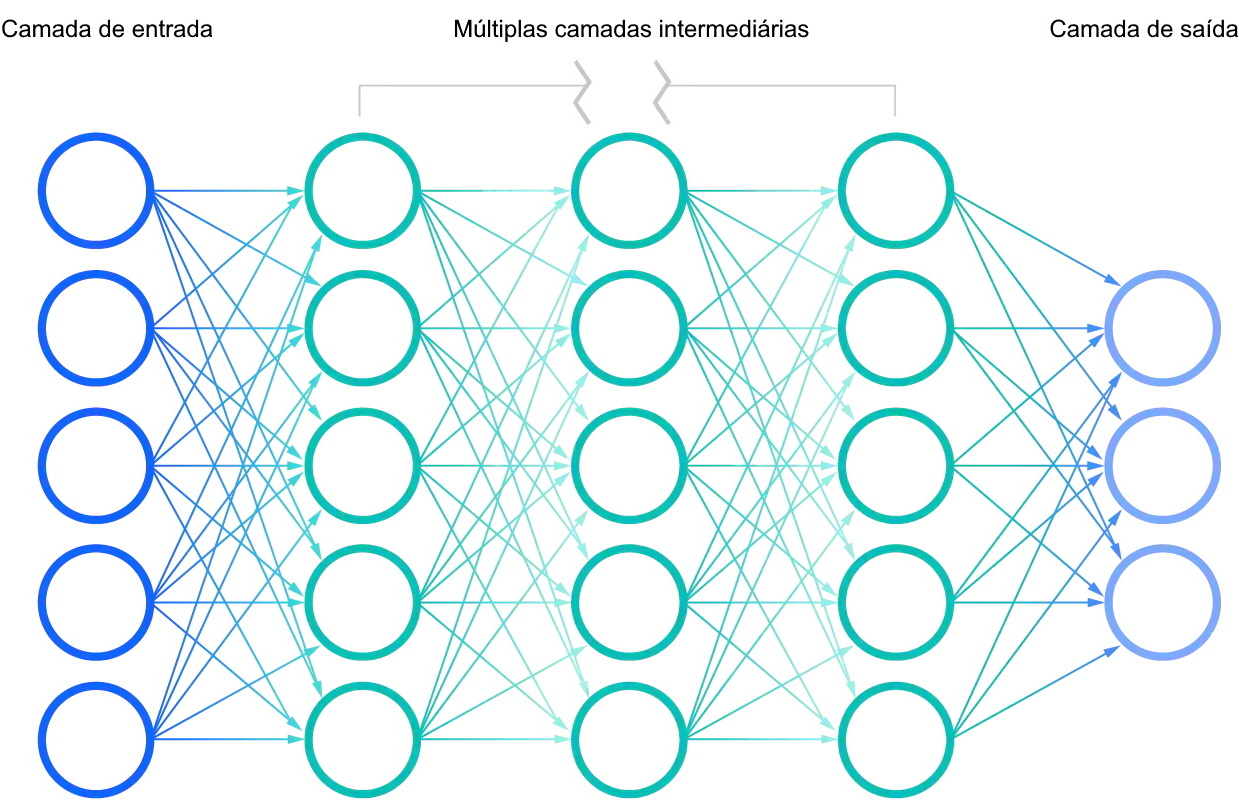
\includegraphics[width=1.0\linewidth]{images/dnn.jpg}
    \label{fig:dnn}
    \fdireta{ibm2020NN}
\end{figure}

Na \autoref{fig:dnn}, cada neurônio é representado por um círculo. 
Durante a criação da rede neural, é designado um peso, bias e função de ativação para cada neurônio. 
Durante o funcionamento, os neurônios enviam informações da esquerda para a direita. No caminho da mensagem, é realizado o cálculo da ativação com base nos seus valores para determinar se é vantajoso ou não que o próximo neurônio receba essa informação \cite{Haykin1998}.

As redes neurais são ótimas ferramentas, mas que precisam passar por um período de treinamento, onde elas aprendem quais são os pesos e limiares de cada conexão para que se tenha o resultado que se espera.
Essa etapa é onde acontece o maior custo computacional por conta da abundante quantidade de cálculos necessários, que aumentam exponencialmente pela quantidade de camadas \cite{lecun2015deep}.

\subsection{Função de ativação}

A função de ativação é um componente fundamental dos neurônios artificiais presentes nas redes neurais. 
É por meio dessa função que os neurônios decidem se devem ou não enviar um sinal para os neurônios da camada seguinte, com base na soma ponderada das entradas recebidas \cite{Goodfellow2016}.  

Em seu livro, \citeonline{haykin2009neural} explica que a função de ativação é responsável por introduzir não-linearidade nas saídas das camadas da rede, permitindo que a rede possa aprender relações não-lineares complexas entre as entradas e as saídas desejadas.
Sem a função de ativação, a rede neural seria uma sequência de operações lineares, o que diminuiria a capacidade de generalização da rede neural e prejudicaria seu desempenho em problemas mais complexos.
Concluindo, a introdução de não-linearidade pela função de ativação permite que a rede neural possa aprender e representar relações não-lineares complexas entre as entradas e as saídas desejadas.

\citeonline{haykin2009neural} ainda explica que a escolha da função de ativação a ser usada depende do tipo de problema e da arquitetura da rede neural. 
Ele destaca que as funções de ativação devem ser escolhidas de modo a permitir que a rede neural alcance o melhor desempenho possível para o problema em questão.

Existem diversas funções de ativação comumente utilizadas em redes neurais. 
Algumas das mais populares são a função sigmóide, a função \sigla{ReLU}{rectified linear unit}, a função \sigla{Tanh}{tangente hiperbólica} tanh e a função \textit{Softmax}.
Outras mais antigas mas que ainda tem utilidade são a função binária e Linear.

A função de ativação binária é uma função de ativação que transforma qualquer valor de entrada (\textit{x}) em uma saída binária, que pode ser apenas 0 ou 1. 
Essa função é frequentemente usada em redes neurais para problemas de classificação binária, onde o objetivo é separar as entradas em duas categorias distintas. Matematicamente, a função de ativação binária é definida na \autoref{eqn:limiar}.
Nessa função, se o valor da entrada \textit{x} e for maior que zero, a saída será 1. 
Caso contrário, a saída será 0.
Embora a função de ativação binária seja simples e eficiente, ela tem algumas limitações. 
Uma das principais limitações é que a função não é diferenciável em x = 0, o que torna difícil a utilização do algoritmo de \textit{backpropagation} para ajustar os pesos da rede neural durante o treinamento. 
Além disso, a função de ativação binária pode ser sensível a ruídos nos dados de entrada, o que pode prejudicar a capacidade da rede neural de generalizar para novos dados.
Por esses motivos, a função de ativação binária é geralmente substituída por funções de ativação mais adequadas para problemas mais complexos

\begin{equation}
\label{eqn:limiar}
    f(x) = \left\{\begin{matrix}
    1 & , x\geq 0\\ 
    0 & , x< 0
    \end{matrix}\right.
\end{equation}


A função de ativação linear é uma função simples que recebe uma entrada e retorna a entrada multiplicada por um peso (\textit{w}) mais um viés (\textit{b}). Matematicamente, ela é definida em \autoref{eqn:linear}. 
Essa função não é muito utilizada em redes neurais profundas, pois sua simplicidade pode levar a problemas de convergência e limitar a capacidade de aprendizado da rede. 
No entanto, ela pode ser útil em algumas situações, como em camadas de saída de redes que precisam produzir valores contínuos e não limitados.

\begin{equation}
\label{eqn:linear}
    f(x) = wx + b
\end{equation}

A função sigmóide é uma função de ativação não-linear comum em redes neurais artificiais. 
Ela tem uma curva em forma de 'S' e mapeia uma entrada (\textit{x}) para uma saída entre 0 e 1, o que é útil para representar probabilidades. 
A equação matemática para a função sigmóide é descrita na \autoref{eqn:sig}.
A função sigmóide é usada principalmente em redes neurais com uma única camada oculta, onde pode ajudar a modelar relações não-lineares entre as variáveis de entrada e saída. 
No entanto, ela tem algumas limitações, como o problema de desvanecimento de gradiente, que pode dificultar o treinamento de redes neurais mais profundas.

    \begin{equation}
    \label{eqn:sig}
    \sigma(x) = \frac{1} {1 + e^{-x}}
    \end{equation}

A função Tanh (\autoref{eqn:tanh}) é uma versão escalonada da função sigmóide (\autoref{eqn:tanhsig}), que busca solucionar os problemas que a função sigmóide possui.
Assim como a função sigmóide, a função Tanh é não linear e possui uma forma de 'S', mas com valores de saída variando de -1 a 1 em vez de 0 a 1, dessa forma possuindo simetria e tanto valores positivos quanto negativos.
Além disso, a função Tanh é simétrica e tem uma região plana em torno de 0, o que significa que, para valores de entrada (\textit{x}) próximos de 0, a função retorna valores próximos de 0.
No entanto, a função Tanh também pode ser propensa a problemas de gradiente desvanecente em redes neurais profundas.
    
\begin{equation}
\label{eqn:tanh}
Tanh(x) = \frac{e^x - e^{-x}}{e^x + e^{-x}} = \frac{1 - e^{-2x}}{1 + e^{-2x}}
\end{equation}

\begin{equation}
\label{eqn:tanhsig}
Tanh(x) = 2\sigma(2x) - 1
\end{equation}

A função de ativação ReLU (\autoref{eqn:relu}) é uma função matemática que transforma um valor de entrada em um valor não negativo.
A função ReLU é uma função não linear e é frequentemente usada como função de ativação em redes neurais artificiais, especialmente em camadas ocultas. 
A principal vantagem da função ReLU é que ela é computacionalmente eficiente e fácil de calcular.

A função ReLU tem uma região plana para valores de entrada (\textit{x}) negativos, onde a função retorna 0. 
Para valores de entrada positivos, a função retorna o próprio valor de entrada. 
A função ReLU é, portanto, uma função de ativação não saturante, o que significa que ela não tem um limite superior no valor de saída. 
Isso pode ser útil para problemas com saídas muito grandes, como detecção de objetos em imagens.
No entanto, a função ReLU pode levar a problemas de "neurônios mortos" em que o neurônio não é ativado para nenhum valor de entrada, resultando em uma rede neural com menos capacidade de aprendizado. 
Para lidar com esse problema, foram propostas variações da função ReLU, como a função \textit{Leaky} ReLU e a função \sigla{ELU}{Exponential Linear Unit}.


\begin{equation}
\label{eqn:relu}
Relu(x) = max(0, x)
\end{equation}

A função de ativação \textit{Softmax} é uma função matemática que transforma um vetor de valores em uma distribuição de probabilidade. 
A função é definida em \autoref{eqn:softmax}, onde onde $x_{i}$ é o i-ésimo valor de entrada e $K$ é a quantidade de valores de entrada.
Dessa forma, a soma é calculada sobre todos os valores de entrada.

\begin{equation}
\label{eqn:softmax}
\sigma(x_i) = \frac{e^{x_{i}}}{\sum_{j=1}^K e^{x_{j}}} \ \ \ for\ i=1,2,\dots,K
\end{equation}

A função \textit{Softmax} é uma função não linear e é frequentemente usada como função de ativação na camada de saída de uma rede neural classificadora. 
A função \textit{Softmax} é usada para transformar as saídas da rede neural em uma distribuição de probabilidade sobre as classes possíveis. 
Cada saída da rede neural é transformada em um valor entre 0 e 1, de modo que a soma de todas as saídas seja igual a 1.

A função \textit{Softmax} é especialmente útil em problemas de classificação multiclasse, onde a rede neural precisa classificar uma entrada em várias classes possíveis. 
A função \textit{Softmax} fornece uma saída normalizada que pode ser interpretada como uma probabilidade de pertencer a cada classe.
No entanto, a função \textit{Softmax} pode ser sensível a valores muito grandes ou muito pequenos de entrada, o que pode levar a problemas de estabilidade numérica. 
Além disso, a função \textit{Softmax} assume que as classes são mutuamente exclusivas e não pode lidar com casos em que uma entrada pode pertencer a mais de uma classe.


\subsection{Feed-forward e Backward propagation}

A propagação feed-forward, ou propagação direta, é um dos principais algoritmos utilizados em redes neurais artificiais para realizar o processamento de dados. 
De forma geral, esse algoritmo consiste em propagar os sinais de entrada da camada anterior para a próxima camada da rede neural, até que o sinal de saída seja obtido na camada de saída. 
Durante essa propagação, os pesos sinápticos são atualizados em cada camada, utilizando um método de otimização, como o gradiente descendente.

Assim como a \autoref{fig:ffp} exemplifica, as entradas %($x_{1}, x_{2}, ..., x_{m}$) 
são processadas pelas primeiras camadas de neurônios % ($\omega_{1}, \omega_{2}, ..., \omega_{m}$)
, que aplicam uma função de ativação na soma dos resultados dos neurônios, para produzir uma saída que é passada para a próxima camada. 
Esse processo é repetido até que a saída final seja produzida pela última camada de neurônios. 
Esse tipo de rede neural é chamado de '\textit{feed-forward}' porque as informações fluem em uma única direção, da entrada para a saída, sem ciclos ou realimentação \cite{Goodfellow2016}.

\begin{figure}[htb]
    \centering
    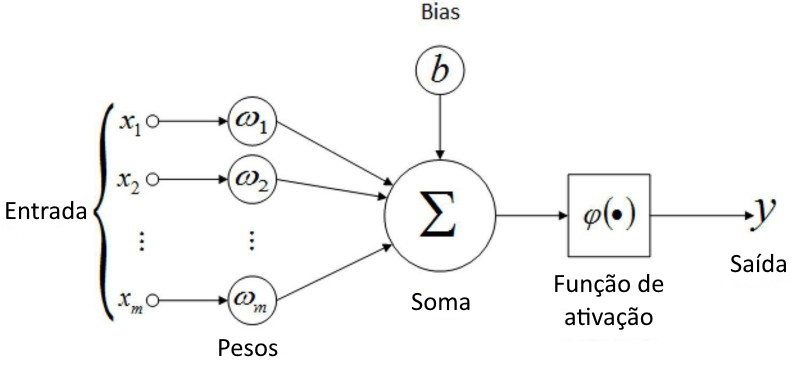
\includegraphics[width=1\linewidth]{TCC UFG/images/aannbias.jpeg}
    \caption{Propagação Feed-Foward.}
    \label{fig:ffp}
    \fadaptada{haykin2009neural}
\end{figure}

De acordo com \citeonline{Goodfellow2016}, a propagação \textit{feed-forward} é a base para muitas arquiteturas de redes neurais, como redes neurais de camadas densas, redes convolucionais e redes recorrentes. 
Além disso, esse algoritmo tem sido amplamente utilizado em várias aplicações de aprendizado de máquina, como reconhecimento de fala, processamento de linguagem natural, classificação de imagens e previsão de séries temporais.

Para realizar a propagação \textit{feed-forward}, é necessário definir a arquitetura da rede neural, que inclui o número de camadas, o número de neurônios em cada camada e a função de ativação utilizada em cada neurônio. 
Segundo \citeonline{Rumelhart1986}, a escolha adequada da arquitetura é crucial para garantir a eficiência e a precisão da rede neural.

Por fim, a propagação \textit{feed-forward} é um processo iterativo e computacionalmente intenso, que pode levar a problemas de convergência lenta ou instável. 
Para contornar esses problemas, vários métodos de regularização, como \textit{dropout} e \textit{L2 regularization}, foram desenvolvidos para melhorar a generalização da rede neural \cite{srivastava2014}.

Propagação para trás, ou \textit{Backward Propagation}, comumente chamado de \textit{backpropagation} é o método de treinamento de redes neurais mais utilizado, podendo ser considerado a essência do treinamento das redes neurais atuais \cite{builtinML}.

O \textit{backpropagation} é um algoritmo de aprendizado de rede neural que funciona de forma contrária ao \textit{feedforward propagation}. 
Enquanto o \textit{feedforward propagation} processa a entrada da rede neural camada por camada, produzindo uma saída, o \textit{backpropagation} começa com a saída da rede e retrocede pelos seus pesos, atualizando-os de acordo com a sua contribuição para o erro da rede \cite{Rumelhart1986}.

O processo de retropropagação é iniciado após o cálculo da saída da rede neural para uma determinada entrada. A partir daí, o gradiente da função de erro é calculado em relação aos pesos da rede. 
Esse gradiente representa a sensibilidade da função de erro em relação a cada peso da rede neural.

Em seguida, o gradiente é propagado de volta pela rede neural, camada por camada, usando a regra da cadeia. 
Em cada camada, o gradiente é usado para calcular a contribuição dos pesos para o erro da rede, permitindo que eles sejam ajustados de acordo com essa contribuição. 
Esse processo é repetido várias vezes até que a rede neural atinja um nível satisfatório de desempenho \cite{Goodfellow2016}.

Em resumo, enquanto o \textit{feedforward propagation} processa a entrada da rede neural e produz uma saída, o \textit{backpropagation} retrocede pelos pesos da rede neural para atualizá-los de acordo com a sua contribuição para o erro da rede.
Essa técnica de aprendizado supervisionado é fundamental para treinar redes neurais profundas e tem sido usada com sucesso em diversas aplicações de aprendizado de máquina \cite{Goodfellow2016}.

\subsection{Sobreajuste e métodos de regularização}

O sobreajuste, ou \textit{overfitting}, é um problema comum em modelos de aprendizado de máquina. 
Ele ocorre quando um modelo é muito complexo, ou profundo no caso das redes neurais convolucionais, e se ajusta muito bem aos dados de treinamento, mas apresenta um desempenho ruim em novos dados. 
Esse problema pode ser evitado com o uso de métodos de regularização.

Existem diferentes métodos de regularização, e um dos mais comuns é o \textit{dropout}. 
A técnica do \textit{dropout} consiste em desativar aleatoriamente alguns neurônios da rede neural durante o treinamento, de modo que a rede seja forçada a aprender a redundância dos dados \cite{srivastava2014}. 
Outra técnica de regularização é a regularização L1 e L2, que adiciona termos de penalidade aos pesos da rede durante o treinamento. 
A regularização L1 adiciona uma penalidade proporcional à soma dos valores absolutos dos pesos, enquanto a regularização L2 adiciona uma penalidade proporcional à soma dos quadrados dos pesos \cite{lecun1998gradient}.

Vale citar que para a redução do \textit{overfitting}, também é necessário que aconteça a escolha adequada de hiperparâmetros, como o tamanho dos lotes ou \textit{batchs}, o número de épocas e a taxa de aprendizado.
Por fim, técnicas de avaliação de desempenho, como validação cruzada e conjunto de validação podem ajudar a identificar e prevenir o \textit{overfitting} \cite{shortImageDeep}.

\subsection{Transferência de aprendizado}

De acordo com \citeonline{Bengio2016}, a transferência de aprendizado se refere à utilização do aprendizado realizado em um contexto de forma a melhorar de forma geral o aprendizado em outro contexto.
Logo, a transferência de aprendizado é uma metodologia para otimização que permite acelerar o processo de aprendizagem e aumentar a performance dos resultados.

Ainda segundo \citeonline{Bengio2016}, na transferência de aprendizado, primeiramente ocorre o treinamento de uma rede neural em uma determinada base de dados para realizar uma tarefa para que então se possa reaproveitar, ou transferir as características aprendidas para uma segunda rede neural que aprende em alguma base da dados para alguma tarefa. 
Esse procedimento tende a funcionar quando as características aprendidas inicialmente são generalizadas ou semelhantes às da outra base de dados.

Esse processo se tornou popular no campo de \textit{deep learning} por diminuir o custo computacional de treinamento, onde há geralmente apenas um pequeno treinamento para aperfeiçoar o modelo pré-treinado para a tarefa determinada, o que requer menor quantidade de dados também \cite{builtintl}. 
De forma prática, essa transferência é tido como a passagem dos pesos de um modelo para outro \cite{builtintl}. 


\section{Redes neurais convolucionais}

\sigla{CNN}{\textit{Convolutional Neural Network}} são uma subclasse de redes neurais profundas, usadas principalmente para análise de conteúdo visual \cite{valueva2020application}. 
A diferença das CNNs em relação a outras redes neurais é que elas não usam o modelo padrão de neurônios independentes uns dos outros, isso acontece pois imagens são matrizes de pixels próximos tendem a se complementar em sentido. 
Para lidar com essa dependência, as CNNs utilizam filtros ou \textit{kernels}, que permitem que a rede aprenda a identificar padrões espaciais em imagens e até temporais em vídeos \cite{lecun1998gradient}.

\begin{figure}[htb]
    \centering
    \caption{Representação genérica de CNN para classificação.}
    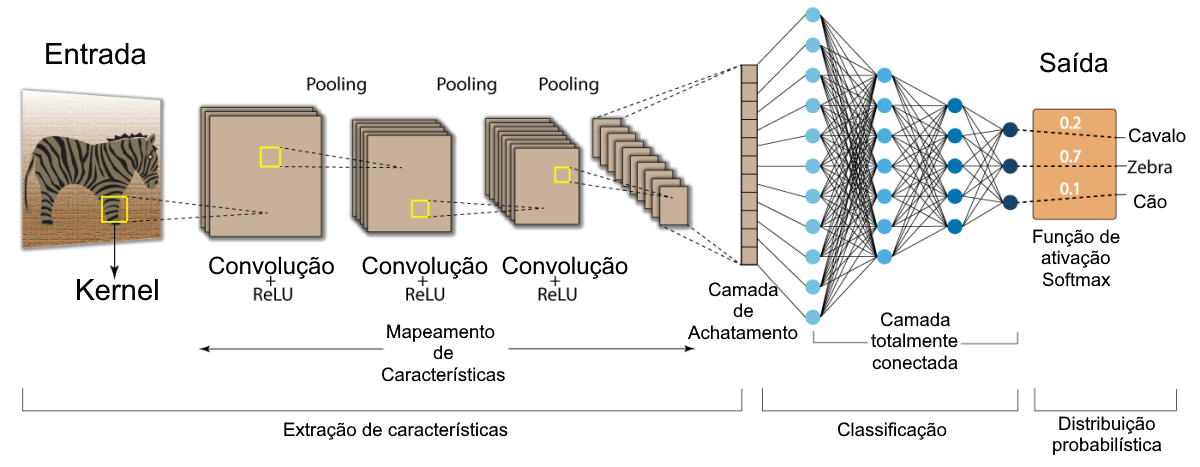
\includegraphics[width=1.0\linewidth]{TCC UFG/images/cnn_example.png}
    \label{fig:genconv}
    \fadaptada{imagemZebra}
\end{figure}

As redes neurais convolucionais são geralmente arquitetadas em blocos. 
Cada bloco é composto por uma ou mais camadas convolucionais, seguidas por camadas de \textit{pooling} e, possivelmente, camadas de normalização. 
Esses blocos são organizados em uma hierarquia, permitindo que a rede neural aprenda gradualmente características cada vez mais complexas. 
A arquitetura em blocos também permite que a rede neural seja projetada de forma modular, permitindo que diferentes arquiteturas sejam criadas a partir de combinações de blocos \cite{simonyan2014very}. 
Alguns exemplos de arquiteturas em blocos amplamente utilizadas em redes neurais convolucionais incluem a VGG, ResNet e Inception.


\subsection{Camada de convolução}

Imagens são estruturas de dados gigantescas, sendo matrizes que guardam até 9 milhões de pixels em uma imagem 4K. 
Logo, as CNNs buscam reduzir essas imagens em uma forma mais fácil de processar sem perder os atributos ou características importantes da imagem \cite{sumitCNN}. 
O processo responsável por essa diminuição é o processo de convolução através de filtros.

A camada de convolução, como o nome já sugere, aplica uma operação de convolução entre os pesos da camada e os dados de entrada para produzir um mapa de características.
Durante a convolução, uma janela deslizante é usada para percorrer toda a imagem de entrada. 
Em cada posição da janela, é feita uma multiplicação elemento a elemento entre os valores da janela e os pesos da camada. 
Em seguida, o resultado dessas multiplicações é somado para produzir um único valor de saída. 
Esse processo é repetido para todas as posições da janela, produzindo um mapa de características.
Esse processo pode ser visualizado na \autoref{fig:conv}.

\begin{figure}[htb]
    \centering
    \caption{Exemplo de convolução.}
    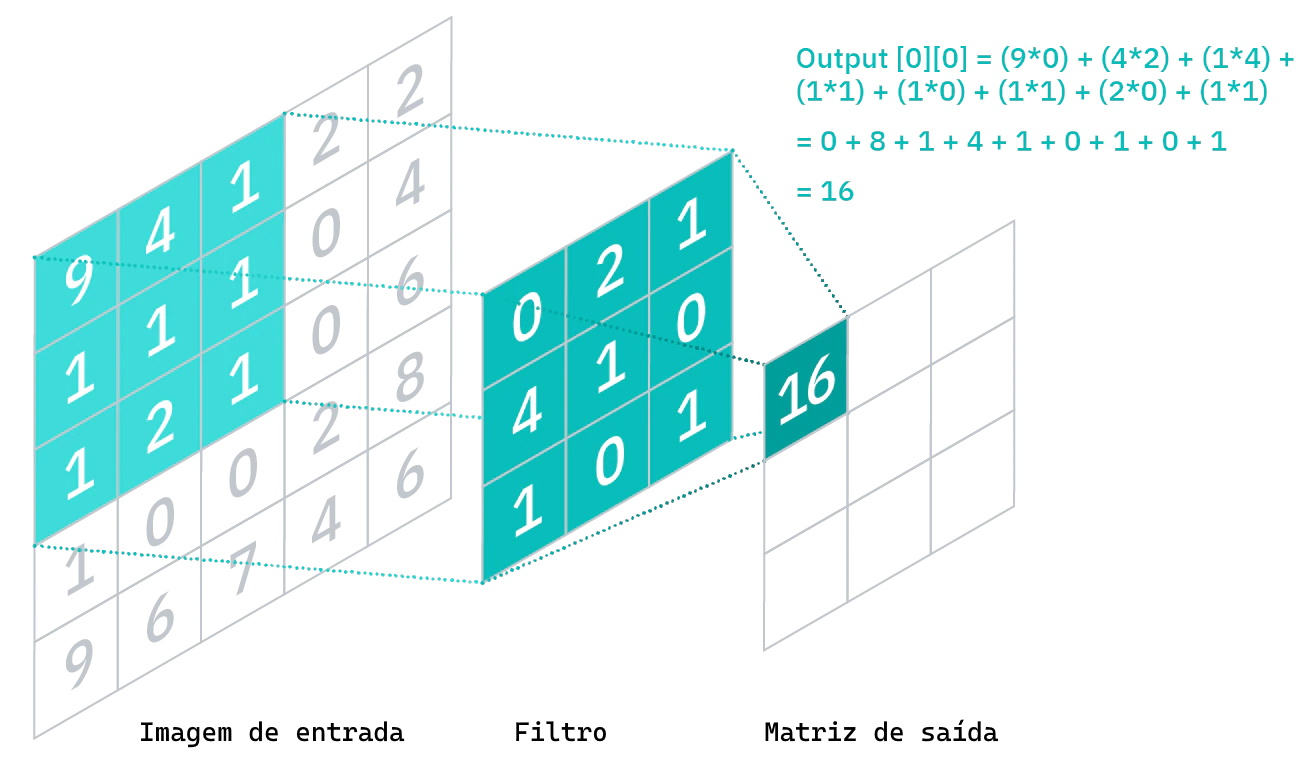
\includegraphics[width=0.8\linewidth]{TCC UFG/images/conv.jpg}
    \label{fig:conv}
    \fadaptada{ibm2020CNN}
\end{figure}

O tamanho da janela é controlado por um parâmetro chamado tamanho do filtro. 
O número de filtros é outro parâmetro que controla quantas características diferentes são extraídas da imagem. 
Cada filtro produz um mapa de características, que é combinado para formar o mapa de características da camada.

Além disso, a camada de convolução pode apresentar outras operações como \textit{padding} e \textit{stride}. 
O \textit{padding} é usado para adicionar uma borda de zeros à imagem de entrada para manter o tamanho do mapa de características de saída. 
O \textit{stride} controla o quanto a janela desliza pela imagem de entrada em cada etapa.


\subsection{Camada de pooling}

A camada de \textit{pooling} é utilizada principalmente para reduzir a dimensionalidade do mapa de características gerado pela camada de convolução, reduzindo o número de parâmetros da rede e evitando o \textit{overfitting} \cite{lecun1998gradient}.
Via de regra, essa camada é aplicada após a camada de convolução, geralmente reduzindo a dimensão espacial do mapa de características e mantendo apenas as características mais importantes. 

Normalmente, são utilizados dois tipos de \textit{pooling}: \textit{max pooling} e \textit{average pooling}.
O mais comum é o \textit{max pooling}, que extrai o valor máximo de cada região do mapa de características.
Já o \textit{average pooling}, extrai a média da região do mapa de características \cite{sumitCNN}.


No entanto, as camadas de \textit{pooling} também podem ter algumas desvantagens, como a perda de informações espaciais e a introdução de distorções na imagem de entrada. 
Essas desvantagens podem ser minimizadas por meio da escolha adequada do tamanho do filtro e do \textit{stride}.

Vale ressaltar que, embora a camada de convolução e a camada de \textit{pooling} tenham o efeito de reduzir a resolução espacial do mapa de características de entrada, elas têm propósitos diferentes na rede neural convolucional.
A camada de convolução tem o objetivo de extrair características e tem como resultado um mapa de características, e nisso como consequência acontece a diminuição da resolução caso não configurado para que não o faça.
Enquanto a camada de \textit{pooling} tem como objetivo principal reduzir a resolução espacial do mapa de características \cite{divaSeg}.

\subsection{Camada de achatamento}

A camada de achatamento tem como função transformar o mapa de características gerado pelas camadas convolucionais em um vetor unidimensional, que pode ser processado pelas camadas totalmente conectadas, ou densas, da rede neural.
Por conta disso, essa camada é geralmente adicionada ao final das camadas convolucionais e antes das camadas densas \cite{lecun2015deep}.

A camada de achatamento é importante porque as camadas densas ou totalmente conectadas requerem uma entrada de vetor unidimensional, enquanto as camadas convolucionais geralmente trabalham com entradas em forma de matriz ou tensor. 
E embora não seja seu foco, a camada de achatamento reduz o número de parâmetros da rede, o que pode ajudar a evitar o \textit{overfitting} e a acelerar o treinamento \cite{lecun2015deep}.


\subsection{Camada totalmente conectada}

Em uma camada totalmente conectada, ou densa, todos os neurônios estão conectados com todos os neurônios da camada anterior. 
Isso significa que cada neurônio de entrada é conectado a cada neurônio de saída. 
Essa conexão densa permite que a camada aprenda representações complexas dos dados e forneça uma saída mais precisa.
Essas camadas geralmente estão localizadas no final da rede neural, depois de uma série de camadas de convolução e de \textit{pooling} \cite{lecun2015deep}. 

Usualmente, a camada densa é utilizada como um classificador, que recebe as características extraídas pelas camadas anteriores e realiza uma classificação ou regressão final \cite{sumitCNN}.
Esse comportamento pode ser visualizado na \autoref{fig:dnn}, onde cada neurônio está ligado a todos os neurônios da próxima camada.

\subsection{Arquiteturas}
\label{dl:arquiteturas}

As arquiteturas em redes neurais convolucionais são as estruturas que determinam como as camadas dessas redes serão organizadas, incluindo o número de camadas, o tipo de camadas, o número de filtros, entre outros aspectos \cite{lecun1998gradient}.

A seguir, são apresentadas algumas das arquiteturas mais conhecidas.

\subsubsection{Arquitetura AlexNet}

% Contextualização do modelo AlexNEt
AlexNet  \cite{alexnetAnalyticsVidhya2021} é uma arquitetura premiada pela competição \textit{ImageNet} de 2012, popularizando a utilização de camadas de convolução cada vez mais profundas, uma de suas principais características, que o tornava um modelo com ótimas performances ao ônus de um considerável aumento no custo computacional \cite{krizhevsky2017imagenet}. 
O modelo conta com oito camadas com cerca de 63 milhões de parâmetros com capacidade de aprendizado, separados em cinco camadas de convolução e três camadas totalmente conectadas onde são utilizados \textit{pooling} e \textit{dropout}, nas saídas de suas camadas é utilizado a função de ativação Relu, exceto na saída final, onde se utiliza da função de ativação \textit{Softmax} \cite{alexnetAnalyticsVidhya2021}. 

A arquitetura AlexNet pode ser vista na \autoref{fig:alexnet}.

\begin{figure}[htb]
    \centering
    \caption{Arquitetura AlexNet.}
    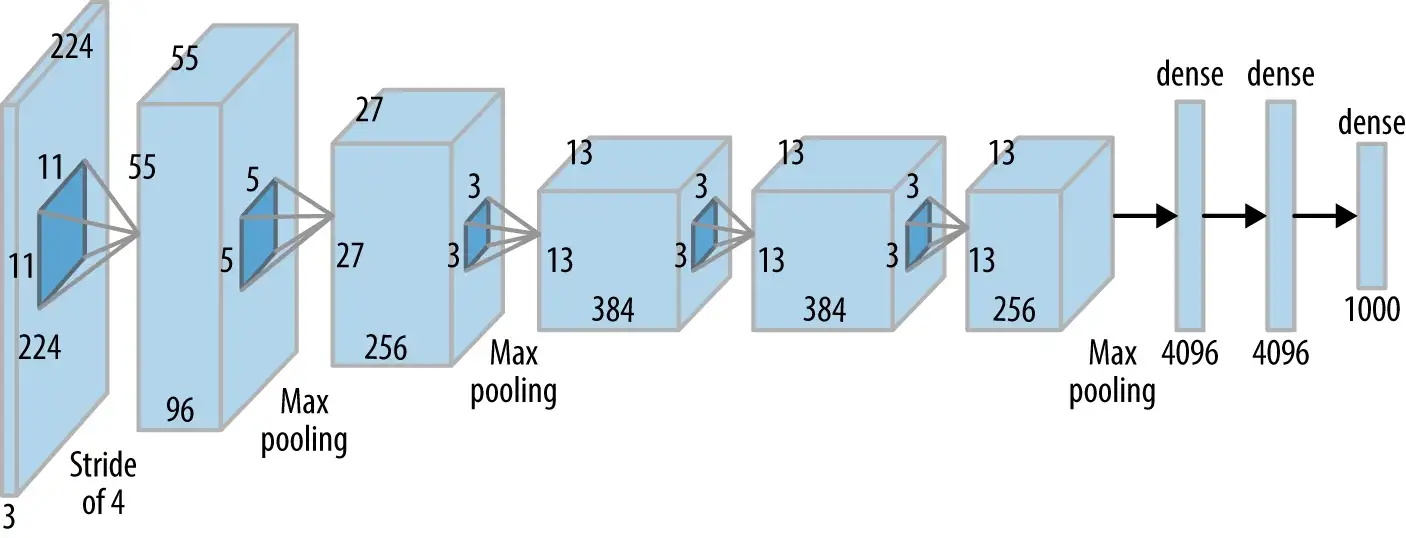
\includegraphics[width=1\linewidth]{images/alexnet.jpg}
    \label{fig:alexnet}
    \fdireta{aqeel2019}
\end{figure}


\subsubsection{Arquitetura VGG}
% Contextualização do modelo VGG16
O grupo de pesquisa \textit{Visual Geometry Group} (VGG) \cite{simonyan2014very}, foi com seus modelo VGG 16 vencedor na modalidade de classificação com localização no desafio \textit{ImageNet} de 2014 e tendo uma boa colocação na de apenas classificação, onde alcançou 92,7\% no teste de acurácia entre a base de dados do \textit{ImageNet}, constituída por 14 milhões de imagens divididas em 1000 classes \cite{ILSVRC15}. 
A principal ideia proposta pelo grupo é a de usar filtros de convolução muito menores, matrizes de tamanho 3x3 com o deslocamento de apenas um pixel por toda a rede neural, sendo bem menor que outros modelos padrões da época como AlexNet \cite{krizhevsky2017imagenet}, que utiliza matriz de convolução de tamanho 11x11 com deslocamento de 4 pixels.
O funcionamento de tal ideia é de utilizar mais camadas para compensar o menor tamanho do filtro, já que no final de cada camada há uma função de ativação, há uma maior utilização de tal processo, fazendo com que a rede se torne mais discriminante  e resultando também no aumento da convergência da rede.
No que diz respeito ao custo computacional, mesmo com aumento na quantidade de camadas, a matriz 3x3 requer menos parâmetros no geral, logo, requer menor potência computacional \cite{GreatLearningVgg16}.


A principal característica do modelo VGG é sua profundidade, com 16 ou 19 camadas convolucionais, que fazem com que o modelo tenha um grande número de parâmetros treináveis. 
Outra particularidade do VGG é que todas as camadas convolucionais têm um filtro 3x3 com o objetivo de reduzir o número de parâmetros e aumentar a capacidade de representação da rede. 
O VGG também utiliza camadas de \textit{max pooling} com filtros de 2x2 para reduzir a resolução espacial das características. 
Além disso, o modelo utiliza camadas densas no final da arquitetura para realizar a classificação final. 
Por causa de sua profundidade e alta capacidade de representação, o modelo VGG alcançou altas performances em diversos conjuntos de dados de imagens, como o \textit{ImageNet} \cite{simonyan2014very}.

Em específico, a VGG16 é constituída por dois blocos iniciais, cada um com duas camadas de convolução seguida pela camada de \textit{max-pooling}, em seguida três blocos intermediários, cada um com três camadas de convolução seguida pela camada de \textit{max-pooling} e para finalizar três camadas densas de convolução.
A arquitetura VGG, em específico o modelo VGG16, pode ser vista na \autoref{fig:vgg16}.

\begin{figure}[htb]
    \centering
    \caption{Configuração do modelo VGG16.}
    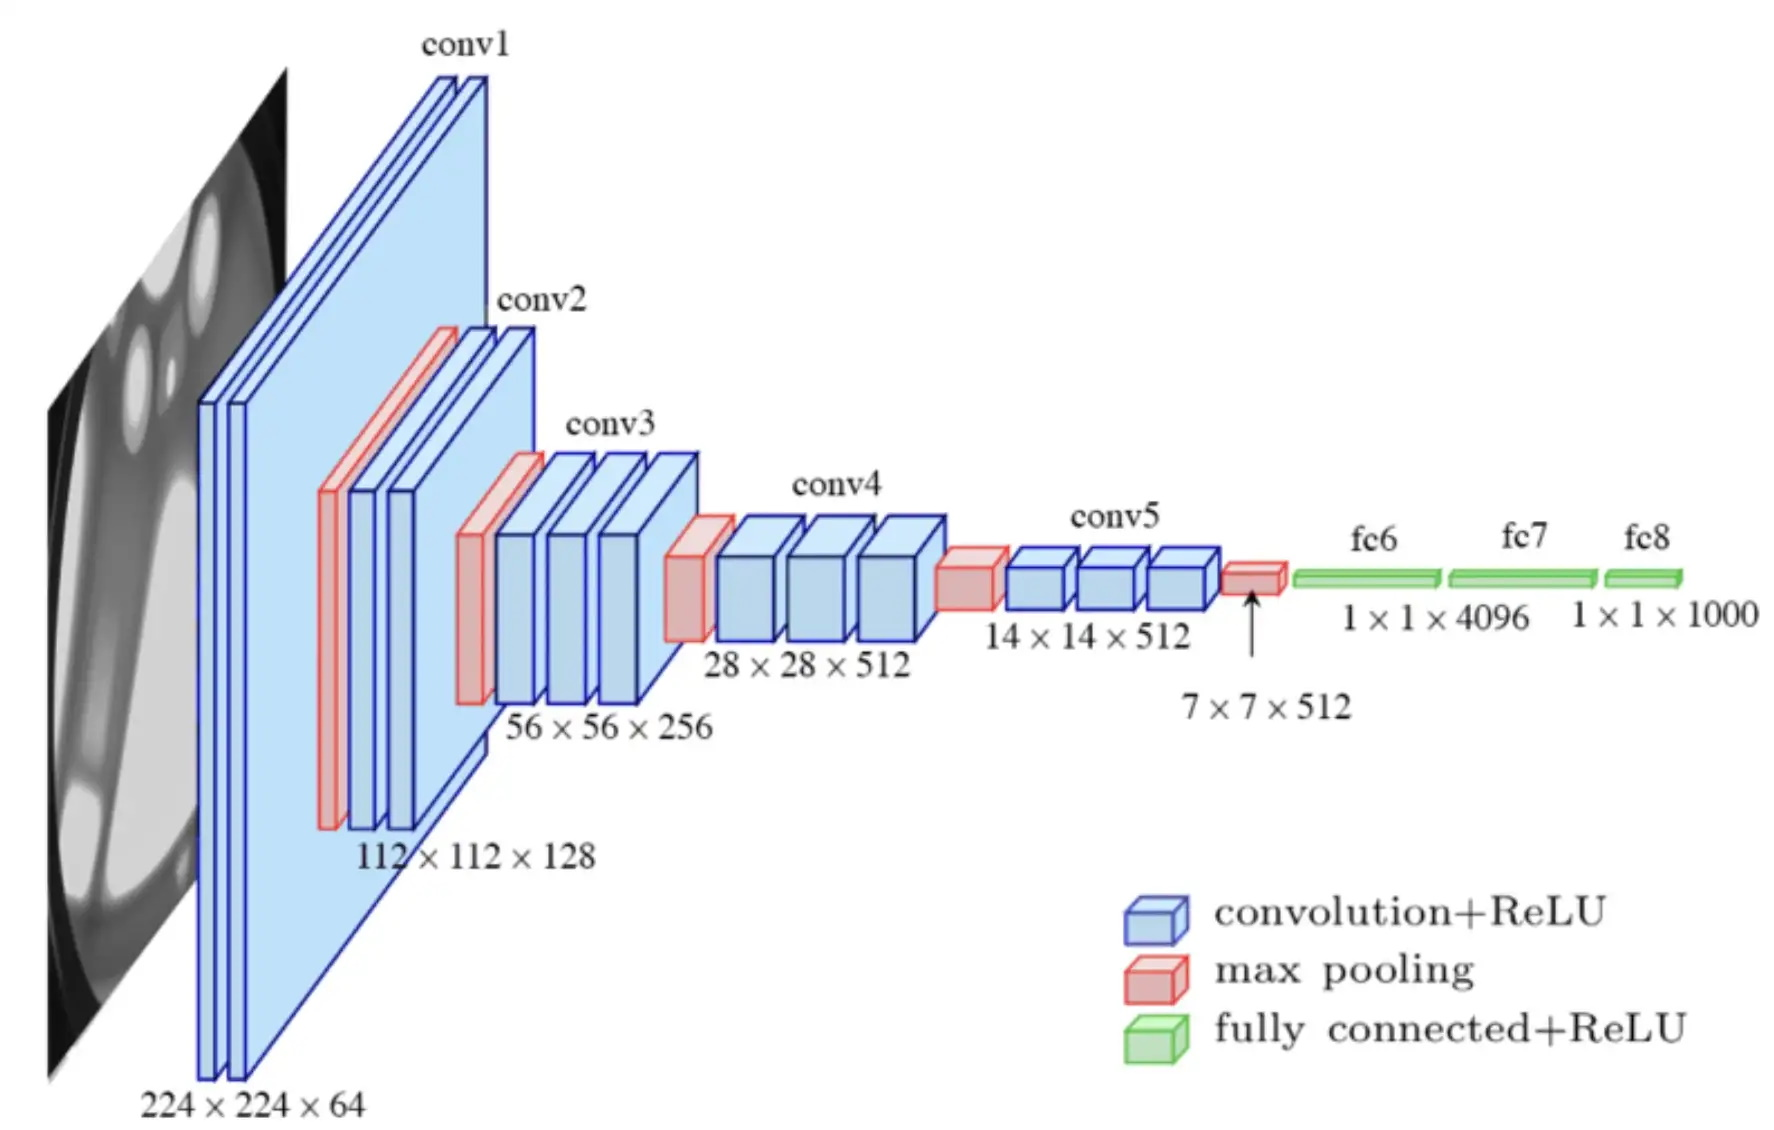
\includegraphics[width=0.8\linewidth]{images/vgg16.jpg}
    \label{fig:vgg16}
    \fdireta{khuyen2021}
\end{figure}



\subsubsection{Arquitetura DenseNet}

% Contextualização do modelo DenseNet
Redes convolucionais densamente conectadas, ou arquitetura DenseNet \cite{huang2017densely} é um modelo recente que promete ser o próximo passo no que diz respeito em aumentar a profundidade das redes convolucionais \cite{PabloDenseNet2018}. 
Após a popularização do aumento da profundidade das camadas convolucionais por conta do modelo AlexNet \cite{krizhevsky2017imagenet} em 2012, houve um constante aumento na profundidade de diversos modelos chegando em números massivos, porém esse aumento no caminho que a informação precisa percorrer desde a camada inicial até a camada final se tornou tão grande que o dado pode ser deturpado e não se tornar nada \cite{PabloDenseNet2018}, além do custo computacional exorbitante. 
Para contornar tais problemas, o DensetNet busca simplificar o modelo de conectividade entre as camadas enquanto garanta que o fluxo de informações não seja perturbado, dessa forma foi utilizado um modelo de reutilização dos extratores de características, realizando conexões que ligam todas camadas diretamente com todas as outras \cite{huang2017densely}. 
Por conta disso o modelo DenseNet precisa de menos parâmetros e elimina a necessidade de camadas redundantes. Se comparado com classificador de uma rede neural genérica que depende dos resultados da última camada de rede, o DenseNet consegue utilizar de forma mais inteligente os resultados já produzidos, obtendo um resultado melhor em performance e precisão.
A \autoref{fig:densenet} ilustra a arquitetura padrão do modelo.

\begin{figure}[htb]
    \centering
    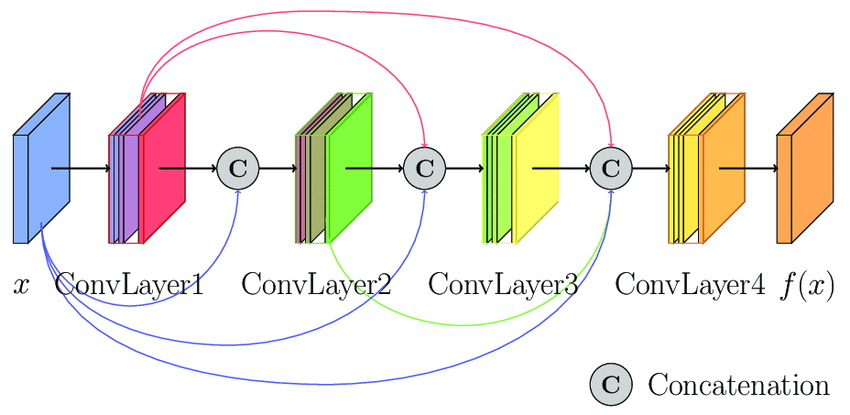
\includegraphics[width=0.8\linewidth]{images/densenet.jpg}
    \caption{Exemplo dos blocos densos em uma DenseNet.}
    \label{fig:densenet}
    \fdireta{mazza2019}
\end{figure}



\subsubsection{Arquitetura Inception V3}
% Contextualização do modelo Inception V3

O modelo \textit{Inception V3}  é uma rede neural convolucional profunda, desenvolvida pela equipe do Google em 2015 \cite{szegedy2015going}. 
O objetivo do modelo é alcançar alta acurácia em tarefas de classificação de imagens, utilizando uma arquitetura que reduz a quantidade de parâmetros e, ao mesmo tempo, mantém um alto desempenho.

Uma das principais características do \textit{Inception V3} é a utilização do módulo de convolução \textit{Inception}, que utiliza diferentes tamanhos de filtros (1x1, 3x3 e 5x5) em paralelo para extrair diferentes características das imagens. 
Além disso, o modelo também utiliza uma camada de \textit{pooling} antes do módulo \textit{Inception} para reduzir a resolução espacial do mapa de características de entrada \cite{szegedy2015going}.

O \textit{Inception V3} também utiliza técnicas de regularização, como o \textit{dropout} e a normalização por lote, para prevenir o \textit{overfitting} durante o treinamento da rede.
O modelo \textit{Inception V3} é um dos modelos mais populares em aplicações de visão computacional, tendo sido utilizado em diversas competições de classificação de imagens, como o \sigla{ILSVRC}{\textit{ImageNet Large Scale Visual Recognition Challenge}} em 2015 e 2016.
O modelo de arquitetura do \textit{Inception V3} pode ser visualizado na  \autoref{fig:inceptionv3}.

\begin{figure}[htb]
    \centering
    \caption{Modelo de arquitetura do Inception V3.}
    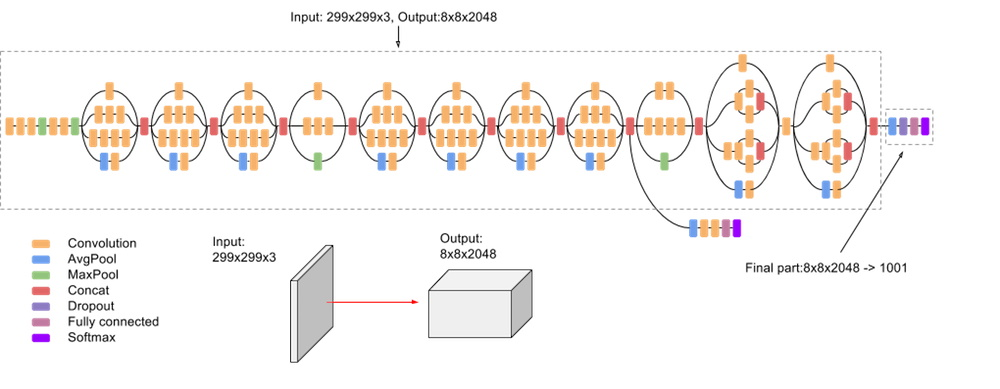
\includegraphics[width=1\linewidth]{images/inceptionv3.jpg}
    \label{fig:inceptionv3}
    \fdireta{googleCloudInceptionv3}
\end{figure}



\subsubsection{Arquitetura ResNet}
% Contextualização do modelo ResNet
\sigla{ResNet}{\textit{Residual neural network}} é uma rede neural convolucional cuja principal característica é ter uma profundidade muito maior que os outros modelos, variando desde 30 camadas até a casa dos milhares \cite{he2016deep}.
A arquitetura ResNET venceu o campeonato \textit{ImageNet} 2015 \cite{deng2009imagenet}, e desde então vem sido o modelo computacional com mais citações \cite{schmidhubermost}. 
Os modelos mais conhecidos desse modelo são ResNet-34, ResNet-50, and ResNet-101 tendo esses nomes por terem profundidade de 34, 50 e 101 respectivamente.

 O principal desafio ao treinar redes profundas é o problema de desvanecimento do gradiente, que ocorre quando o gradiente se torna tão pequeno que a rede não consegue aprender com as atualizações de peso. 
 O ResNet resolve esse problema introduzindo conexões residuais entre as camadas da rede, permitindo que a informação de entrada flua diretamente para camadas posteriores \cite{Vanshika2021}.
 Esse processo pode ser observado na \autoref{fig:camada_residual}, onde a entrada \textit{x} flui diretamente para uma camada posterior.

Teoricamente, a utilização das conexões residuais faz com que os parâmetros aprendidos sejam guardados e repassados para as camadas futuras, dessa forma, mesmo que aconteça os problemas como a dissipação de gradiente, haverá uma camada posterior que receberá de volta os parâmetros aprendidos \cite{Vanshika2021}. 
O agrupamento dessas camadas, desde onde há o começo de um atalho, até a camada conectada por este atalho é chamado de bloco residual \cite{he2016deep}.
O bloco em questão é composto por duas camadas convolucionais, seguidas por uma operação de adição que permite que a ativação da camada anterior seja adicionada à ativação atual. 
Essa operação de adição permite que a rede aprenda apenas as diferenças entre a ativação atual e a ativação anterior, ao invés de ter que re-aprender toda a representação da entrada \cite{he2016deep}.

Por fim, o ResNet  consegue utilizar blocos residuais que contêm múltiplas camadas convolucionais em paralelo, permitindo que a rede aprenda múltiplas representações de uma mesma entrada \cite{Vanshika2021}.


\begin{figure}[htb]
    \centering
    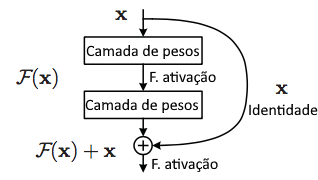
\includegraphics[width=0.5\linewidth]{TCC UFG/images/adap_cama_res.png}
    \caption{Exemplo de bloco residual.}
    \label{fig:camada_residual}
    \fadaptada{he2016deep}
\end{figure}
 
